\section{EAP Method Definition}
We want to encapsulate our extended zero-knowledge authentication system defined in \S\ref{label:protocol-design}  as an EAP method in the EAP framework we've explored in \S\ref{section:eap}.
To achieve this we must define a new EAP method, which consists of messages exchanged between the \textit{peer} and the \textit{authenticator}, their data formats and how processes for handling them.

\paragraph{Terminology}
In this section we will be using EAP terminology as described in \S\ref{section:eap}, which uses different names to describe parties involved, as the ones used in our system architecture in \S\ref{label:protocol-design} or as in the ZKP protocol in \S\ref{zkp-qrp}.
The two parties in EAP are called the peer and the authenticator, where the peer is authenticating with the authenticator.
To draw parallels between our system architecture, where we use the names \textit{user} and \textit{authentication system}, the peer is the user and the authenticator is the authentication system.
In the ZKP protocol names \textit{prover} and \textit{verifier} are used, the peer is the prover, and the authenticator is the verifier.


\subsection{Method Definition}

To define an EAP method we need to break down our authentication system to EAP messages representing interactions between between the prover and the verifier.
Each message defines its data format, the sender and recipient processes and local state changes.

The symbols $n, s, w, y, z$ have the same definition as in the system architecture described in \S\ref{label:protocol-design}.
In our architecture we assumed the modulus $n$ and salt $s$ are known by the prover, however the EAP method needs to facilitate the discovery of this data.

The EAP method consists of two message pairs, the \textit{setup message} pair exchanged sent once and the \textit{verification message} pair is exchanged $m$ times.
The first pair is used to facilitate the \textit{setup phase} of the \textit{authentication process} and the second pair to facilitate the \textit{verification phase}.
It should be noted that both message pairs are not one-to-one match with the communication described in our architecture in \S\ref{zkp-qrp} . 
Doing a one-to-one match would create three message pairs with empty spaces in some response and request data.
In order to save on space we've managed to compress the authentication process into two message pairs, by interlacing some data transfer of the \textit{verification} phase in the response of the \textit{setup} phase and the response of the preceding verification phase, we'll explore how exactly we achieve this when defining the data formats of each message.

The authenticator can optionally use the \textit{identity} type EAP message the query the identity of the peer, this might be useful to locate the unique salt belonging to the peer.

To end the method, the authenticator sends a \textit{success} message after successfully authenticating the peer, or a \textit{failure} message otherwise.

\begin{figure}[h]
	\centering
	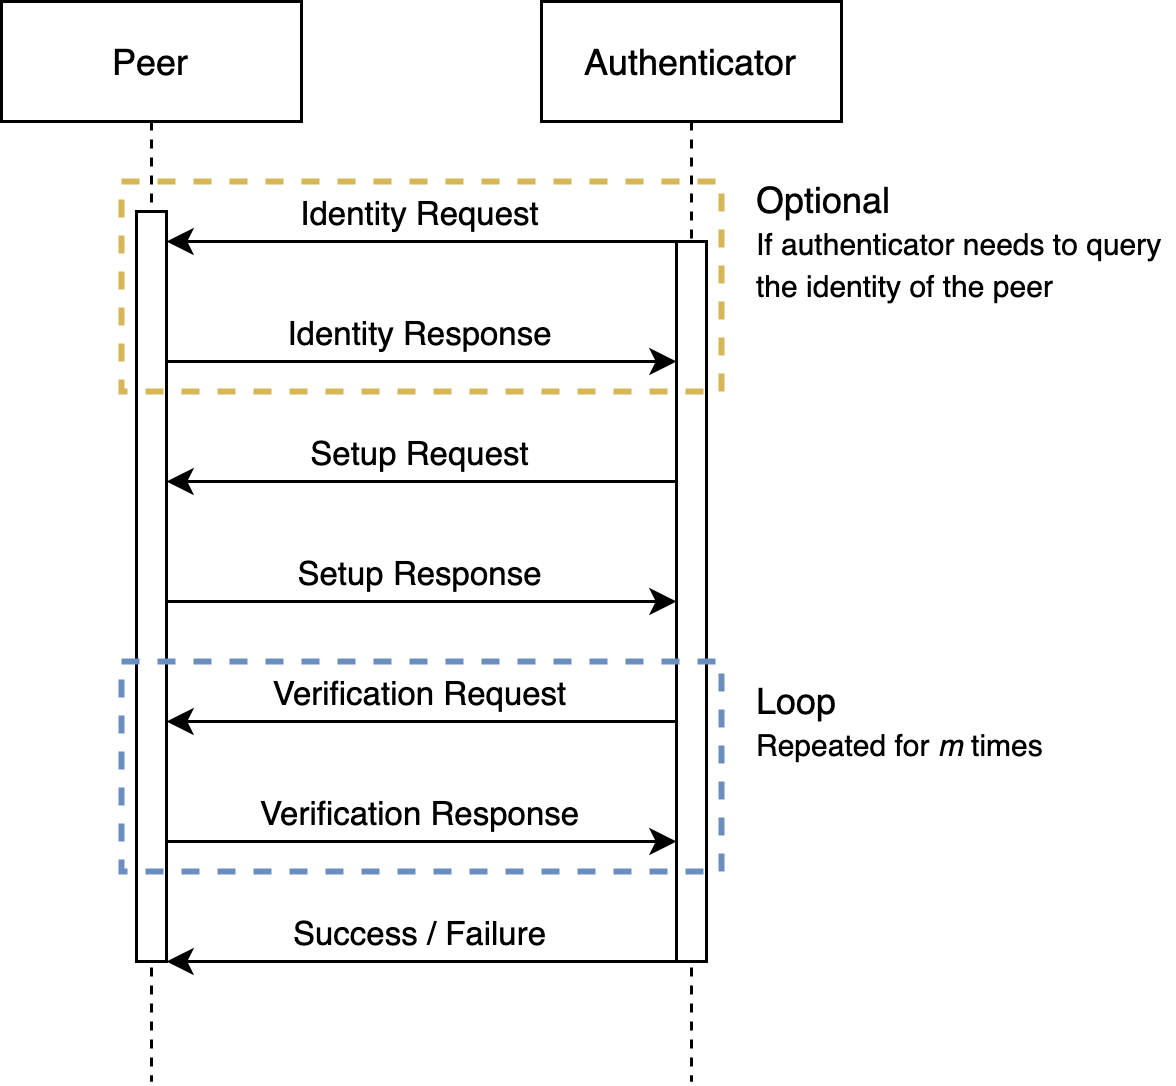
\includegraphics[width=12cm]{images/EAP_Method.png}
	\caption{EAP Method Execution}
	\label{fig:eap-method-protocol}
\end{figure}

%\subsubsection{Message Format}
Each EAP method is identified by the \textit{type} field of the EAP message, our method is represented by the type 84.
The message pair of the EAP method is identified by the \textit{sub-type} field.
\medskip
\begin{itemize}
	\item Setup (Sub Type 1)
	\item Verification (Sub Type 2)
\end{itemize}

\subsection{Setup Message Pair}

%\paragraph{Request}
%
%\paragraph{Response}

\subsubsection{Request} Message is used to deliver the salt $s$ and semiprime modulus $n$ to the peer.

\paragraph{Data Format}

\begin{center}
\begin{tabular}{|c|c|c|c|c|}
	\hline
	Length (Octets) & ... & 1 & $4 \le k \le 255 $ & $64 \le j$\\
	\hline
	Field Type & ... & Salt Length & Salt & Semiprime Modulus\\
	\hline
\end{tabular}
\end{center}

\begin{description}
	\item[Salt Length] A single octet for the length of the \textit salt field in octets.
	\item[Salt] A random salt value, should be from 4 octets to 255 octets long.
The max length is determined by the largest number able to be encoded in the \textit {salt length} field.
	\item[Semiprime Modulus] Fills the rest of the message to the length specified by the \textit{length} field in the EAP header. 
Should be at least 64 octets (512 bits).
\end{description}

\paragraph{Request Handling} When a request is received, the peer computes the secret $w$ using the password $p$ the salt $s$ with the pre-determined hashing function $H$.
$$w = H(p, s)$$
Secret value $w$ should be stored stored in memory by the peer. 
Next the peer should pick a random integer $u$ from field $Z^*_n$, and store it in memory and then compute the control value $y = u^2 \Mod{n}$.
The control value $y$ is included in the response message.
\bigskip
\\
In order to locate the unique salt in a system with multiple peer identities, the authenticator can optionally use the \textit{identity} method (Type 1) to query the identity of the peer.


\subsubsection{Response}
The response transmits the control value $y$ to the authenticator to be used in the verification process.

\paragraph{Data Format}

\begin{center}
\begin{tabular}{|c|c|c|}
	\hline
	Length (Octets) & ... & $k$ \\
	\hline
	Field Type & ... & Control Value $y$\\
	\hline
\end{tabular}
\end{center}

\bigskip

\begin{description}
	\item[Control Value] Computed by the peer, where $y = u^2 \Mod{n}$ and $u \leftarrow_R \mathbb{Z}^*_n$.
\end{description}

\paragraph{Response Handler}
The authenticator should store the $y$ control value locally to be used when verifying the proof.

\subsection{Verification Message Pair}
This message pair is continuously exchanged repeatedly until the authentication is concluded.
The purpose of this message is to deliver data to the authenticator that can be used to assert the peers knowledge of $w$, if at any point the assertion fails the authentication was unsuccessful.
Only after $m$ iterations, or after the authenticator reaches a set confidence of $1 - 2^{-m}$ in the proof is the authentication successful.

To make our method more efficient, we reduce the number of exchanged messages between the parties by interlacing some data between iterations.
On round $i$, the response contains data required for round $i+1$.

\subsubsection{Request}
The authenticator generates random bit $b$ stores it locally, and sends it to the peer.
\paragraph{Data Format}

\begin{center}
\begin{tabular}{|c|c|c|}
	\hline
	Length (Octets) & ... & $1$ \\
	\hline
	Field Type & ... & Random Bit $b$\\
	\hline
\end{tabular}
\end{center}

\begin{description}
	\item[Random Bit] A single-bit $b$, at the right-most place. 1 octet long.
\end{description}

\paragraph{Request Handling}
The peer computes the proof $z = uw^b \Mod{n}$, with the bit $b$ received in the request.

Additionally the peer generates the control value $y$ for the next ($i+1$) round of the verification phase, it generates a random integer $u_{i+1}$ from field $Z^*_n$, and store it in memory and computes the control value $y_{i+1} = u_{i+1}^2 \Mod{n}$.

\subsubsection{Response}

The response transmits the proof $z$ and the control value $y_{i+1}$ to the authenticator, who verifies the proof and makes a decision on how to proceed.
\paragraph{Data Format}

\begin{center}
\begin{tabular}{|c|c|c|c|c|}
	\hline
	Length (Octets) & ... & $1$ & $k $ & $j$\\
	\hline
	Field Type & ... & Proof Length & Proof $z$ & Control Value $y_{i+1}$\\ %TODO: Witness, check if this is the correct term?
	\hline
\end{tabular}
\end{center}

\begin{description}
	\item [Proof Length] A field one octet in length. Determines the length of the Proof field in octets.
	\item [Proof] Value $z$ computed by the peer, verified by the authenticator.
	\item [Control Value] Value $y_{i+1}$, required to verify the proof of the $(i+1)$-th round.
\end{description}

\paragraph{Response Handling}
The authenticator should verify the proof by asserting that $z^2 \equiv yx^b \Mod{n}$.
If the assertion fails the a \textit{failure} message must be sent to the peer, otherwise a \textit{success} message must be sent if the peer was successfully verified $m$ times.
If that is not the case, the $y_{i+1}$ is stored by the authenticator and a new random bit $b$ is send to the peer in the message request.

%\subsection{Optimisations}
%EAP is a lock-step protocol, the authenticator and the peer exchange request and response messages.
%
%A naive mapping of PBA-ZKP-QRP messages to EAP packets yields 3 new request/response pairs. 
%We can reduce the amount of new pairs to 2 instead of 3, by interlacing data shared in each pair.
%This way we obtain a faster performance by reducing the number of packet needed to be exchanged.
%
%\subsubsection{Naive Map}
%
%\begin{center}
%	\begin{tabular}{c|rcl}
%	Pair & Peer  & $\leftrightarrow$ & Authenticator \\
%	\hline
%	1 & & $\xleftarrow{s, n}$ &\\
%	&& $\xrightarrow{\textvisiblespace}$&\\
%	\hline
%	2 & & $\xleftarrow{\textvisiblespace}$&\\
%	&& $\xrightarrow{y}$&\\
%	\hline
%	3 & & $\xleftarrow{b}$&\\
%	&& $\xrightarrow{z}$&\\
%	\hline
%	\end{tabular}
%\end{center}
%
%\paragraph{Pair 1} Exchanged once after the authenticator obtaining the peers identity. The authenticator sends the salt $s$ and semiprime modulus $n$ to the peer, in order for the peer to compute the private input $w$. 
%Peers response serves as an acknowledgement of a successful setup.
%
%This pair corresponds to the \textit{setup} part of the protocol.
%
%\paragraph{Pair 2} The authenticator requests the peer to generate the \textit{square} value $y$ and share it in the response.
%
%This pair corresponds to the ZKP-QRP part of the protocol and is repeated for $m$ times. %TODO: Update the terminology to use ZKP-QRP everwhere
%
%\paragraph{Pair 3} The authenticator requests the peer to compute the \textit{witness} value $z$, with the value of the random bit $b$ in the request data.
%
%This pair corresponds to the ZKP-QRP part of the protocol and is repeated for $m$ times.
%
%\paragraph{Performance}
%With this mapping a successful protocol run of $m$ iterations with a probability of error of $2^{-m}$, would require a minimum of $4m + 3$ packet exchanges.
%
%\bigskip
%
%\begin{center}
%	\begin{tabular}{r|l}
%		Packets exchanged & Type\\
%		\hline
%		2 & Pair 1\\
%		$2m$ & Pair 2\\
%		$2m$ & Pair 3\\
%		1 & Type 2 (Success)\\
%	\end{tabular}
%\end{center}
%
%\subsubsection{Interlaced Data Mapping}
%
%\begin{center}
%	\begin{tabular}{c|rcl}
%	Pair & Peer  & $\leftrightarrow$ & Authenticator \\
%	\hline
%	1 & & $\xleftarrow{\text{s, n}}$ &\\
%	&& $\xrightarrow{y_1}$&\\
%	\hline
%	2 & & $\xleftarrow{b}$&\\
%	&& $\xrightarrow{z, y_{n+1}}$&\\
%	\hline
%	\end{tabular}
%\end{center}
%
%\paragraph{Pair 1} Exchanged once after the authenticator obtains the peers identity. 
%The authenticator sends the salt $s$ and semiprime modulus $n$ to the peer, in order for the peer to compute the private input $w$.
%Peer computes the square value $y$ and sends it in the response.
%
%The main difference with the naive mapping is that the peer responds prematurely with $y$, instead of in the response to naive pair 2. %TODO: Reword, weird sentence
%This is possible and valid, because the semiprime modulus value $n$ required to compute $y$, is provided in the pair 1 request.
%
%\paragraph{Pair 2}
%The authenticator already has the square value $y$, and sends a request with a random bit $b$. 
%The peer computes sends the \textit{witness} $z$ and the square value $y_{n+1}$, used in the next iteration of the protocol
%
%This is possible because the computation of square value $y$ is only dependent on the modulus $n$, which is provided in the request pair 1.
%
%\paragraph{Performance}
%With this mapping a successful protocol run of $m$ rounds with an error rate $2^{-m}$, would require a minimum of $2m + 3$ packet exchanges.
%
%\begin{center}
%\begin{tabular}{r|l}
%	Packets exchanged & Type\\
%	\hline
%	2 & Pair 1\\
%	$2m$ & Pair 2\\
%	1 & Type 2 (Success)\\
%\end{tabular}
%\end{center}
%
%Comparing the performance of both mappings, the interlaced mapping requires half as many exchanges for the same $m$ rounds of protocol.
%
%$$\lim_{1 \rightarrow \infty} \frac{2m + 3}{4m + 3} = \frac{1}{2}$$
%
%\bigskip
%\subsection{Security}
%EAP PB-ZKP-QRP is resistant to passive attacks to over-the-wire information, eavesdropping, active attacks and offline attacks with pre-computed tables/rainbow tables.
%
%The protocol does not enable mutual authentication, nor helps in deriving a session key that can be used for data encryption.
